\documentclass[conf]{new-aiaa}
%\documentclass[journal]{new-aiaa} for journal papers
\usepackage[utf8]{inputenc}

\usepackage{graphicx}
\usepackage{amsmath, amsfonts}
\usepackage{commath}
\usepackage[version=4]{mhchem}
\usepackage{siunitx}
\usepackage{subfigure}
\usepackage{longtable,tabularx}
\usepackage{xcolor}
\setlength\LTleft{0pt} 

\graphicspath{{./figs/}}

\title{Comparing Optimization and Estimation Techniques for Low-Thrust Spacecraft Rendezvous}

\author{Andrew Cox, Mike Sparapany, Collin York, Waqar Zaidi}
\affil{Department of Aeronautics and Astronautics, Purdue University, West Lafayette, IN}

\begin{document}

\maketitle

\begin{abstract}
Low-thrust technologies offer efficient mass usage which can lower spacecraft mass and, thus, mission costs. However, due to the small forces generated by low-thrust engines, long-duration burns are required to significantly alter a spacecraft path. Accordingly, low-thrust trajectory design must incorporate additional variables to describe the thrust vector during the burn duration. The solution to this higher-dimensional trajectory design problem is often obtained via optimal control where the thrust vector constitutes the set of control variables. In this study, a rendezvous scenario between a low-thrust-equipped spacecraft and an uncontrolled ``mothership'' is considered. Uncertainties in the spacecraft position, velocity, and thrust vectors are mitigated via estimation algorithms and a mass-optimal trajectory is obtained that satisfies the natural dynamics and mission-imposed constraints. Several techniques for optimization and estimation are investigated and their effects on the optimal solution are discussed.
\end{abstract}

\section{Nomenclature}

{\renewcommand\arraystretch{1.0}
\noindent\begin{longtable*}{@{}l @{\quad=\quad} l@{}}
$\mathbf{\Phi}$ & state transition matrix\\
$\alpha$ & thrust pointing angle\\
$\lambda_i$ & costate\\
$\theta$ & spacecraft longitude angle\\
$\theta'$ & target longitude angle\\
$\mu$ & Earth gravitational parameter\\
$\vec{\psi}$ & terminal constraint vector\\
$\phi$ & terminal cost\\
$\mathbf{A}$ & Jacobian matrix\\
$\vec{F}_g$ & gravity force vector\\
$\vec{F}_{lt}$ & low-thrust force vector\\
$H$ & Hamiltonian\\
$I_{sp}$ & specific impulse\\
$J$ & optimization cost\\
$L$ & Lagrangian\\
$T$ & thrust magnitude\\
$\hat{e}$ & rotating frame unit vector\\
$g_0$ & Earth mean gravitational acceleration\\
$\hat{i}$ & inertial frame unit vector\\
$m$ & spacecraft mass\\
$n'$ & target mean motion\\
$r$ & spacecraft orbital radius\\
$r'$ & target orbital radius\\
$u$ & control state\\
\end{longtable*}}

\section{Introduction}
Rendezvous of a chaser spacecraft with a target spacecraft in a predetermined orbit is a common problem in spaceflight operations. Spacecraft mass is frequently minimized during such operations to reduce overall mission expenditures. Advancements in low-thrust propulsion technology facilitate these minimizations by transforming propellant mass into a propulsive force more efficiently than other technologies. However, due to the small accelerations delivered by low-thrust systems, significant burn durations are required to alter the course of the spacecraft. Accordingly, low-thrust trajectory design must incorporate variables to describe the thrust vector in addition to the usual variables that describe a spacecraft state. The following proposed analysis attempts to blend these two traditional spaceflight problems and determine optimization and estimation techniques that allow rendezvous using low-thrust propulsion systems.

\section{Problem Definition}
{\color{blue} Note: This is likely more verbose than it needs to be; we can trim later}

The rendezvous problem includes two vehicles: the target and the ``chaser,'' refered to hereafter simply as the spacecraft. The target moves on a circular orbit about the Earth with an orbital radius $r'$ and is located by angle $\theta'$ relative to the inertial $x$-axis, $\hat{i}_x$, as depicted in Figure \ref{fig:frames}.
\begin{figure}[ht!]
	\centering
	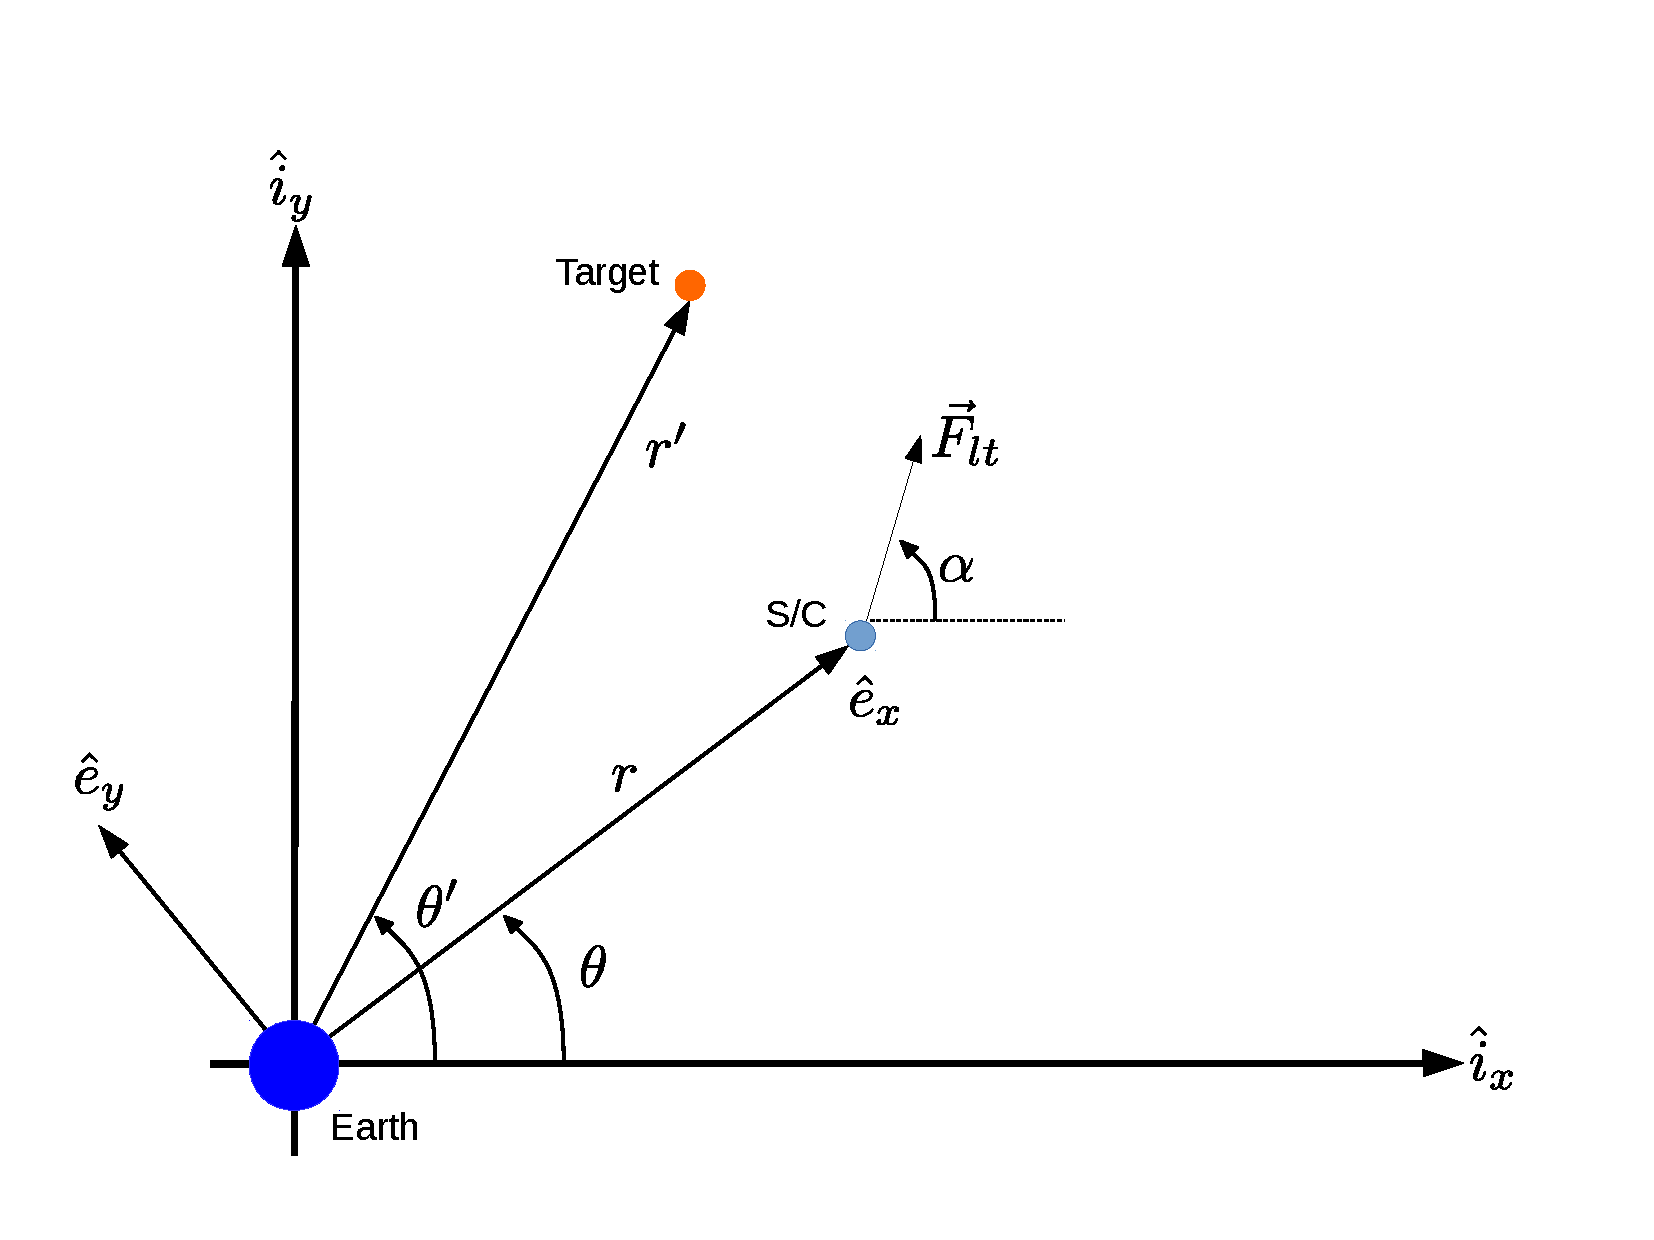
\includegraphics[width=0.7\textwidth]{Frames.pdf}
	\caption{The spacecraft (S/C) and target are located relative to the Earth}
	\label{fig:frames}
\end{figure}
As the target orbit is circular, the angle may be represented as a simple function of time,
\begin{equation}
	\theta' = \theta'_0 + n't\,,
\end{equation}
where $\theta'_0$ locates the initial target position, $t$ is time, $n'$ is the target mean motion,
\begin{equation}
	n' = \sqrt{\frac{\mu}{r'^3}}\,,
\end{equation}
and $\mu$ is the gravitational parameter associated with Earth, $\mu = 3.986\times 10^5$ km$^3$/s$^2$. The chaser vehicle, i.e., the spacecraft, is located in an arbitrary orbit about the Earth with instantaneous radius $r$ and angle $\theta$. Let the $\hat{e}$ frame rotate with the spacecraft such that $\hat{e}_x$ points from the Earth to the spacecraft, $\hat{e}_z = \hat{i}_z$, and $\hat{e}_y$ completes the right-handed set.

\subsection{Equations of Motion}
Two forces are modeled to define the spacecraft motion. First, gravity is modeled via the inverse-square relationship,
\begin{equation}
	\vec{F}_g = \frac{-\mu m}{r^2} \hat{e}_x\,,
\end{equation}
where $m$ is the spacecraft mass. Additionally, a low-thrust force is applied to the spacecraft and is modeled as
\begin{equation}
	\vec{F}_{lt} = T\left( \cos\alpha \hat{i}_x + \sin\alpha \hat{i}_y \right)\,,
\end{equation}
where $T$ represents the thrust magnitude and $\alpha$ orients the thrust vector relative to the inertial $x$-axis. Apply Newton's law to describe the spacecraft acceleration,
\begin{equation}
	m\ddot{\vec{r}} = \sum \vec{F}\,.
\end{equation}
Let the spacecraft position vector be $\vec{r} = r \hat{e}_x$. Accordingly, the spacecraft acceleration vector is
\begin{equation}
	\ddot{\vec{r}} = \left( \ddot{r} - r \dot{\theta}^2 \right) \hat{e}_x + \left( 2 \dot{r} \dot{\theta} + r \ddot{\theta} \right) \hat{e}_y\,.
\end{equation}
Substitute this relationship into Newton's law to write two equations of motion,
\begin{align}
	\ddot{r} &= r\dot{\theta}^2 - \frac{\mu}{r^2} + \frac{T}{m} \left( C_{\alpha} C_{\theta} + S_{\alpha} S_{\theta} \right)\,,\\
	\ddot{\theta} &= -2\frac{\dot{r}\dot{\theta}}{r} + \frac{T}{mr} \left( S_{\alpha} C_{\theta} - C_{\alpha} S_{\theta} \right)\,.
\end{align}
An additional equation describes the spacecraft mass,
\begin{equation}
	\dot{m} = \frac{-T}{I_{sp} g_0}\,,
\end{equation}
where $I_{sp}$ is the engine specific impulse, and $g_0$ is the mean Earth gravitational acceleration, $g_0 = 9.80665$ m/s$^2$. Define a state vector, $\vec{x}~=~\begin{Bmatrix}r & \theta & \dot{r} & \dot{\theta} & m \end{Bmatrix}^T$, and let the governing equations be
\begin{equation}
	\dot{\vec{x}} = \begin{Bmatrix} 
		\dot{r}\\ \dot{\theta}\\
		r\dot{\theta}^2 - \frac{\mu}{r^2} + \frac{T}{m} \left( C_{\alpha} C_{\theta} + S_{\alpha} S_{\theta} \right)\\
		-2\frac{\dot{r}\dot{\theta}}{r} + \frac{T}{mr} \left( S_{\alpha} C_{\theta} - C_{\alpha} S_{\theta} \right)\\
		-T/(I_{sp} g_0)
	\end{Bmatrix}
	\label{eq:dynamics}
\end{equation}\,.
The Jacobian matrix, which relates variations in the state variables to variations in their derivatives, is frequently useful in optimization and estimation processes and facilitates the construction of the state transition matrix. Let the Jacobian be represented by the matrix
\begin{equation}
	\mathbf{A} = \dpd{\dot{\vec{x}}}{\vec{x}} = \begin{bmatrix}
		0 & 0 & 1 & 0 & 0\\
		0 & 0 & 0 & 1 & 0\\
		\dot{\theta}^2 + 2\mu/r^3 & \frac{T}{m}\left( -C_{\alpha}S_{\theta} + S_{\alpha}C_{\theta} \right) & 0 & 2r\dot{\theta} & -\frac{T}{m^2}\left( C_{\alpha}C_{\theta} + S_{\alpha}S_{\theta} \right)\\
		\frac{2\dot{r}\dot{\theta}}{r^2} - \frac{T}{mr^2}\left( S_{\alpha}C_{\theta} - C_{\alpha}S_{\theta} \right) & -\frac{T}{mr} \left( S_{\alpha}S_{\theta} + C_{\alpha}C_{\theta} \right) & -2\dot{\theta}/r & -2\dot{r}/r & -\frac{T}{m^2r} \left( S_{\alpha}C_{\theta} - C_{\alpha} S_{\theta} \right)\\
		0 & 0 & 0 & 0 & 0
	\end{bmatrix}\,.
\end{equation}
Accordingly, the state transition matrix, $\mathbf{\Phi}(t_1,~t_0)$, that relates variations in $\vec{x}(t_0)$ to variations at some later state $\vec{x}(t_1)$ is governed by the differential equation,
\begin{equation}
	\dot{\mathbf{\Phi}} = \mathbf{A \Phi}\,.
\end{equation}

\subsection{Optimization Problem}
The goal of the rendezvous problem is to move the spacecraft to the location of the target while minimizing expended mass or, equivalently, maximizing final mass. Accordingly, the optimization problem is
\begin{equation}
	\underset{\alpha}{\text{min}} ~J = -m(t_f)\,,
\end{equation}
subject to the dynamics in Equation \eqref{eq:dynamics}, the initial conditions
\[
	r(t_0) = r_0\,, \qquad \theta(t_0) = \theta_0\,, \qquad \dot{r}(t_0) = \dot{r}_0\,, \qquad \dot{\theta}(t_0) = \dot{\theta}_0\,, \qquad m(t_0) = m_0\,, t_0 = 0\,,
\]
and the terminal constraints
\begin{equation}
	\vec{\psi} = \begin{Bmatrix}
		r(t_f) - r'\\
		\theta(t_f) - \theta'_0 - n t_f\\
		\dot{r}(t_f)\\
		\dot{\theta}(t_f) - n
	\end{Bmatrix} = \vec{0}
\end{equation}

\subsection{Solution via Indirect Optimization}
The standard form of the cost function in the Bolza problem is given by
\begin{equation*}
	J = \phi(x(t_f),~t_f) + \int\limits_{t_0}^{t_f} L(\vec{x}, \vec{u}, t) \dif t\,.
\end{equation*}
Thus, the rendezvous problem is formulated such that $\phi = -m(t_f)$, $L=0$, and $\vec{u} = \{\alpha \}$. Define the Hamiltonian,
\begin{align}
	H &\equiv L + \vec{\lambda}^T \dot{\vec{x}} \nonumber\\
	H &= \lambda_1 \dot{r} + \lambda_2 \dot{\theta} + 
		\lambda_3 \left[ r \dot{\theta}^2 - \frac{\mu}{r} + \frac{T}{m} \left( C_{\alpha} C_{\theta} + S_{\alpha} S_{\theta} \right) \right] + \nonumber\\
		&\qquad\qquad \lambda_4 \left[ -2\frac{\dot{r}\dot{\theta}}{r} + \frac{T}{mr} \left( S_{\alpha} C_{\theta} - C_{\alpha} S_{\theta} \right) \right] - \lambda_5 \frac{T}{I_{sp} g_0}\,.
\end{align}
Apply the Euler-Lagrange equations to find the costate derivatives,
\begin{align}
	\dot{\lambda}_1 &= -\dpd{H}{r} = -\lambda_3\left[ \dot{\theta}^2 + \frac{2\mu}{r^3} \right] - \lambda_4 \left[ \frac{2 \dot{r}\dot{\theta}}{r^2} - \frac{T}{mr^2}\left( S_{\alpha} C_{\theta} - C_{\alpha} S_{\theta} \right) \right]\,,\\
	\dot{\lambda}_2 &= -\dpd{H}{\theta} = -\lambda_3 \frac{T}{m} \left( -C_{\alpha} S_{\theta} + S_{\alpha} C_{\theta} \right) - \lambda_4 \frac{T}{mr} \left( -S_{\alpha} S_{\theta} - C_{\alpha} C_{\theta} \right)\,,\\
	\dot{\lambda}_3 &= -\dpd{H}{\dot{r}} = -\lambda_1 + \lambda_4 \frac{2 \dot{\theta}}{r}\,,\\
	\dot{\lambda}_4 &= -\dpd{H}{\dot{\theta}} = -\lambda_2 - 2\lambda_3 r \dot{\theta} + \lambda_4 \frac{2\dot{r}}{r}\,,\\
	\dot{\lambda}_5 &= -\dpd{H}{m} = \lambda_3 \frac{T}{m^2} \left( C_{\alpha} C_{\theta} + S_{\alpha} S_{\theta} \right) + \lambda_4 \frac{T}{rm^2} \left( S_{\alpha} C_{\theta} - C_{\alpha} S_{\theta} \right)\,.
\end{align}
Similarly, the optimal control law is derived via
\begin{equation}
	u^* = u~\left| \dpd{H}{\alpha} = 0 \right. \quad \to \quad \dpd{H}{u} = \lambda_3 \frac{T}{m} \left( -S_{\alpha} C_{\theta} + C_{\alpha} S_{\theta} \right) + \lambda_4 \frac{T}{mr} \left( C_{\alpha} C_{\theta} + S_{\alpha} S_{\theta} \right) = 0\,.
	\label{eq:dHdu}
\end{equation}
To simplify notation, let $\gamma$ represent the thrust pointing angle in the rotating frame, i.e., $\gamma = \alpha - \theta$. Then, assuming $T$ and $m$ are nonzero throughout the optimization, Equation \eqref{eq:dHdu} simplifies to
\begin{equation}
	\dpd{H}{u} = -\lambda_3 S_{\gamma} + \frac{1}{r}\lambda_4 C_{\gamma} = 0 \quad \to \quad r \tan \gamma = \frac{\pm \lambda_4}{\pm \lambda_3}\,.
\end{equation}
To resolve the sign ambiguity, evaluate the second partial derivative,
\begin{align}
	\dpd[2]{H}{\alpha} &= -\lambda_3 \frac{T}{m} \left(C_{\alpha} C_{\theta} + S_{\alpha} S_{\theta} \right) + \lambda_3 \frac{T}{mr} \left(-S_{\alpha} C_{\theta} + C_{\alpha} S_{\theta} \right) > 0\\
	&= \frac{T}{m} \left[ -\lambda_3 C_{\gamma} - \lambda_4 \frac{1}{r} S_{\gamma} \right] > 0\,.
\end{align}
The thrust and mass are always positive ($T/m > 0$), thus, choose the negative coefficients for $\lambda_3$ and $\lambda_4$. The sine and cosine functions are then rewritten in terms of the costates,
\begin{align}
	S_{\gamma} &= \frac{-\lambda_4}{\sqrt{r^2\lambda_3^2 + \lambda_4^2}}\,,\\
	C_{\gamma} &= \frac{-r \lambda_3}{\sqrt{r^2\lambda_3^2 + \lambda_4^2}}\,.
\end{align}
Boundary conditions are available from the terminal constraints and terminal cost. The variation in each terminal constraint is given by
\begin{equation}
	\dif \psi_i = \dpd{\psi_i}{\vec{x}_f} \dif \vec{x}_f + \dpd{\psi_i}{t_f} \dif t_f\,.
\end{equation}
Accordingly, the following relationships result,
\begin{align}
	\dif r_f &= 0\,,\\
	\dif \theta_f &= n \dif t_f\,,\\
	\dif \dot{r}_f &= 0\,,\\
	\dif \dot{\theta}_f &= 0\,.
\end{align}
A similar relationship is available for the terminal cost variation,
\begin{equation}
	\dif \phi = \dpd{\phi}{\vec{x}_f} \dif \vec{x}_f + \dpd{\phi}{t_f} \dif t_f\,.
\end{equation}
Substituting the relationships for this problem yields the equation,
\begin{equation}
	\dif \phi = -\dif m_f\,.
\end{equation}
This variations are all incorporated into the \textit{transversality condition},
\begin{equation}
	H^*(t_f) \dif t_f - \vec{\lambda}_f^T \dif \vec{x}_f + \dif \phi = 0\,.
\end{equation}
The resulting relationship is given by
\begin{align}
	H^*_f \dif t_f - \lambda_{2,f} \dif \theta_f - \lambda_{5,f} - \dif m_f &= 0 \nonumber\\
	\left[ H^*_f - \lambda_{2,f} n \right] \dif t_f - \left[1 + \lambda_{5,f} \right] \dif m_f &= 0\,.
\end{align}
Since neither $\dif t_f$ nor $\dif m_f$ are zero, each coefficient must independently evaluate to zero to satisfy the transversality condition. Two boundary conditions result:
\[ \lambda_{2,f} = H^*_f/n\,, \qquad \lambda_{5,f} = -1 \]
With these boundary conditions, the two-point boundary value problem is well-defined:

\begin{align*}
	\dot{r} &= \dot{r}\\
	%
	\dot{\theta} &= \dot{\theta}\\
	%
	\ddot{r} &= r\dot{\theta}^2 - \frac{\mu}{r^2} - \frac{T}{m} \frac{r \lambda_3}{\sqrt{r^2\lambda_3^2 + \lambda_4^2}}\\
	%
	\ddot{\theta} &= -2\frac{\dot{r}\dot{\theta}}{r} - \frac{T}{mr} \frac{\lambda_4}{\sqrt{r^2\lambda_3^2 + \lambda_4^2}} \\
	%
	\dot{m} &= -T/(I_{sp} g_0)\\
	%
	\dot{\lambda}_1 &= -\lambda_3\left[ \dot{\theta}^2 + \frac{2\mu}{r^3} \right] - \lambda_4 \left[ \frac{2 \dot{r}\dot{\theta}}{r^2} + \frac{T}{mr^2} \frac{\lambda_4}{\sqrt{r^2\lambda_3^2 + \lambda_4^2}} \right]\,,\\
	%
	\dot{\lambda}_2 &= 2\frac{T}{m} \frac{\lambda_3 \lambda_4}{\sqrt{r^2\lambda_3^2 + \lambda_4^2}}\,,\\
	%
	\dot{\lambda}_3 &= -\lambda_1 + \lambda_4 \frac{2 \dot{\theta}}{r}\,,\\
	%
	\dot{\lambda}_4 &= -\lambda_2 - 2\lambda_3 r \dot{\theta} + \lambda_4 \frac{2\dot{r}}{r}\,,\\
	%
	\dot{\lambda}_5 &= -\frac{T}{m^2} \frac{r \lambda_3^2}{\sqrt{r^2\lambda_3^2 + \lambda_4^2}} - \frac{T}{rm^2} \frac{\lambda_4^2}{\sqrt{r^2\lambda_3^2 + \lambda_4^2}}\,.
\end{align*}
\[ r(t_0) = r_0\,, \qquad \theta(t_0) = \theta_0\,, \qquad \dot{r}(t_0) = \dot{r}_0\,, \qquad \dot{\theta}(t_0) = \dot{\theta}_0\,, \qquad m(t_0) = m_0\,, \qquad t_0 = 0\,, \]
\[ r_(t_f) = f'\,, \qquad \theta(t_f) = \theta'_0 + nt_f\,, \qquad \dot{r}(t_f) = 0\,, \qquad \dot{\theta}(t_f) = n\,, \qquad \lambda_2(t_f) = \frac{H^*_f}{n}\,, \qquad \lambda_5(t_f) = -1\]
\end{document}

\subsection{Estimation}

\section{Trade Studies}
What are we comparing? How? What are the expected results?

\section{Results}

\section{Concluding Remarks}
A conclusion section is not required, though it is preferred. Although a conclusion may review the main points of the paper, do not replicate the abstract as the conclusion. A conclusion might elaborate on the importance of the work or suggest applications and extensions. \textit{Note that the conclusion section is the last section of the paper that should be numbered. The appendix (if present), acknowledgment, and references should be listed without numbers.}

\section{Contributions}
Who did what?

\bibliography{sources.bib}

\end{document}
